\documentclass[12pt,twoside]{third-rep}

\usepackage{url}
\usepackage{pslatex}

\usepackage{listings}
\lstset{
  language=Python,
  numbers=left,
  breaklines=true,
  basicstyle=\ttfamily
}
\lstMakeShortInline[columns=fixed]|

\usepackage{titlesec}
\usepackage{hyperref}
\usepackage{enumitem}
\usepackage{fancyhdr}
\usepackage{subcaption}

\usepackage{graphicx}
\graphicspath{{img/}}

\pagestyle{fancy}
\fancyhf{}
\fancyhead[LE,RO]{\rightmark}
\fancyhead[RE,LO]{\thepage}
\renewcommand{\headrulewidth}{0pt}

\titleformat{\chapter}[display]
  {\normalfont\bfseries}{}{0pt}{\Large}

\title{Automatic Birdsong Recognition}

\author{Victor F. Lampreia Rodrigues}

\supervisor{Dr. Andrea Schalk}

\reportyear{2017}

\abstractfile{tex/abstract.tex}
%\thanksfile{thx.tex}

\begin{document}

\dotitleandabstract

\tableofcontents
\listoffigures
\listoftables

\chapter{INTRODUCTION}

\section{Motivation}
Automatic birdsong recognition is far from solved outside of controlled
environments or with heavy user input.
A system which can recognize species from birdsong from a wide variety of
species is an exciting application of signal processing, computer vision and
machine learning technologies.
Such software would be beneficial to the bird enthusiasts and environmental
health associations, and others.

\section{Goals}
The primary aim of this project is to research and develop potential methods
for automatic birdsong recognition, with little to no user interaction.
The program should recognize up to 50 distinct bird species from field recordings
provided by arbitrary sources around the world.
The recordings should not have any form of rigorous quality control such as
recordings performed under controlled environments.
Sample selection may be performed to ensure quality levels are kept at a
reasonably normalised level, as many recordings are expected to contain
excessive amounts of noise.

For the purposes of this project, bird songs will be solely considered, and calls
will not be used.
This limits the complexity of the classification requirements as calls tend to
differ significantly to songs.

\section{Potential Approaches}
is this section needed?

All approaches in this section deal with either the waveform image of a birdsong
recording, a spectrogram of the recording, or both.

\subsection{DTW / archetypes}
previous student used waveform and DTW to match against an archetype waveform.

\subsection{Image recognition}
spectral shapes etc
some have used image recognition to match templates representative of specific
bird species to identify birds in a recording using it's spectrogram.

\subsection{Spectral Analysis}
The mean spectral frequency and energy information in spectrograms may give some
clues as to which species of bird is vocalizing.

\subsection{Pitch Tracking}
forgot what this was called, was used for whalesong recognition.
may not work well for birdsong recognition due to relative pitches etc?


\section{Our Approach}
Our initial approach is inspired by similar sound recognition problems.
Such problems include the recognition of voice, music, animals vocalisations
including whale song, calls, and so on.
It is observed that these problems, while similar in nature, differ in practice.
This is mainly due to the nature of the sound being analysed, as well as
domain knowledge of the structure.

For example, the acoustics of human voice is well studied, and patterns are
easily identified today.
Specialised methods for analysing voice recordings exist, including intonation
etc etc \textbf{add more}.
we have a mapping, we know the words, we dont speak bird noises

Music recognition is trivial in the case of identifying pure reproductions,
the main challenge in this area being noise reduction and distortion compensation.
Music can be easily identified using statistical methods to compare pitch
variations along the duration of the recording.
Bird song however contains many variations and transpositions within the same
species which make it difficult to find an archetypal sequence of pitch
variations.\\

Some approaches to these problems are essentially spectrographic image recognition
tasks, where elements common to specific labels are searched for within a target
example spectrogram.
The simplicity and success of such solutions has driven the direction of this
project.

Our approach uses a combination of computer vision and machine learning
techniques to construct a fully automatic recognition system.
Standard image processing methods are used to process spectrograms and extract
sections of song which may be used to identify a particular species, much like
how an orthonologist visually inspects the song spectra.
These sections are then matched against new samples to be classified through a
multi-class machine learning algorithm.

move bulk of subsections to appendices

\subsection{Process Overview}
The project is divided into four discrete parts.
These follow the logical flow of data in the system:
\begin{enumerate}
  \item \textbf{Collection:}
    Data is sourced from field recordings done in uncontrolled environments.
    The variety provides a good estimate of real-world performance and
    introduces many quality related issues.

  \item \textbf{Preparation and selection:}
    Recordings are filtered and selected to maintain reasonable quality levels.
    Spectrograms are then derived from the recordings.
    This is now the representation that is used throughout the program until
    the feature vector is constructed.

  \item \textbf{Preprocessing and feature extraction:}
    Noise is reduced as much as possible to identify key regions of interest
    within the spectrogram image.
    These are extracted as templates and cross-correlated against other
    recording spectrograms to form a feature vector.

  \item \textbf{Classification and evaluation:}
    The resulting data is then fed to a classifier and evaluated using techniques
    designed to reduce statistical bias.
\end{enumerate}

Each of these procedures are described in detail in their respective sections.
A few of these sections discuss possible alternatives or improvements to the
developed mechanisms.

Performance is an equally important aspect of this project, as such some
analysis is performed on the cost of key stages.
A report on this is available in appendix xyz.

\subsection{Architecture Overview}
\textbf{diagram of key sections}

Due to the experimental nature of the project, a rigorous architecture has not
been designed ahead of time.
The codebase evolved through several iterations 

\subsubsection{Data persistence}


\subsection{Implementation Technologies}
All code is written in Python 2.7.
Libraries used include:
\begin{itemize}
  \item open-CV 2.0
\end{itemize}


\chapter{WORKING DATA}

This project bases all mechanisms on one single birdsong representation, the
source field recordings.
This section describes the data used, how it is collected, and prepared for
usage within the program.


\section{Data Source: Xeno-Canto}

Xeno-Canto \parencite{xenocanto} provides over 353830 recordings of 9728
individual species.
Recordings consist of both calls and song, uploaded by arbitrary users, and
therefore may originate from any part of the world, may vary extremely in
terms of quality, and content.

Recordings vary in duration, ranging from 1 to 20 minutes each.
The content may be densely packed, with multiple birds vocalising simultaneously,
or sparse with long durations of silence.
Additionally, multiple species may be present in a single recording, however
higher quality recordings tend to contain a singly identifiable species.

Xeno-canto provides all audio as dynamic MP3.
These are normalised as described in Section~\ref{sec:prep}

\subsection{Metadata}
Xeno-canto provides the following metadata with each recording:
\begin{itemize}[noitemsep]
  \item Date and time
  \item Recording location
  \item Species recorded
  \item Existence of other species
\end{itemize}

This program only makes use of the prominent species tagged in the recording.
Although not used in our implementation, the location of the recording could be
used to improve the accuracy of the classifier, as some species are restricted
to certain parts of the world.
Including this information in the feature set is very likely to provide a
good accuracy by itself, but perhaps without precision.
It could be used however to narrow down the set of possible species, so long as
special care is taken to account for migratory patterns.


\subsection{Automatic Sample Retrieval}
Manually selecting and downloading recordings is a time-consuming process.
A public API does not exist for Xeno-canto, therefore we developed a web scraper
specifically for automatic retrieval in |Python 2.7| using the |lxml| package.

The scraper allows the user to filter samples on species and on recording quality
before downloading a sample by examining the metadata present in the HMTL.
Filtering may be done by exclusion or selection.

When continuous fetching is desired, an interval may be set in order to reduce
strain on Xeno-Canto's servers.
Once an interval is set, the scraper will continuously download samples
at the specified rate until it has been interrupted by the user.\\

The scraper was ran throughout the course of development, for an approximate
accumulated time of 40 hours, with an average interval of 60 seconds between
downloads.
2211 audio samples were collected in total.


\section{Preparation}\label{sec:prep}
Before the data can be further processed and used, some basic preparation
must be done to normalise the data.
This section discusses the transformative steps and the end representation that
the program will work with from the initial state until classification.

\subsection{Resampling}
Because the source recordings vary in format, we normalise these to the following
format:
\begin{itemize}[noitemsep]
  \item \textbf{Format:} Raw WAV
  \item \textbf{Audio channels:} 1
  \item \textbf{Bit depth:} 16-bits
  \item \textbf{Sample rate:} 22050 Hz
\end{itemize}

If a recording is found to have more than a single channel, all but the left
channel are discarded.
It is unclear whether discarding a channel is better than summing them.
While summing retains all information, it may also introduce further noise.
Conversely, it is allso possible for the left channel to have a worse signal to
noise ratio than the right.
The number of multi-channel recordings is low enough for this not to be much
of an issue.

Sample rates are reduced to lower the memory and processing demands of
analysing all 45 hours of audio.
Our image recognition approach holds greater importance to the general shape
of individual vocalisations in spectrograms, rather than high time-frequency
details.
Because of this, the sample rate reduction is found to have no significant
reductions in classification quality.

The recording duration is left unaltered, so durations may differ from sample to
sample.

The FFmpeg \parencite{ffmpeg} program is used to convert all source material.
We have written a shell script to make this procedure fully automatic, executable
when new recordings have been sourced.


\subsection{Spectrogram Representation}
A spectrogram is a visualisation of a sound as energy in the frequency spectrum
in function of time.
This allows us to intuitively visualise the shape of a sound as a 2d image.
Figure~\ref{fig:sgram_pcm} shows how the spectrogram representation retains
amplitude information from a waveform, while exposing the frequency composition
of the waveform.

\begin{figure}[!htb]
  \centering
  \begin{subfigure}[b]{1.0\textwidth}
    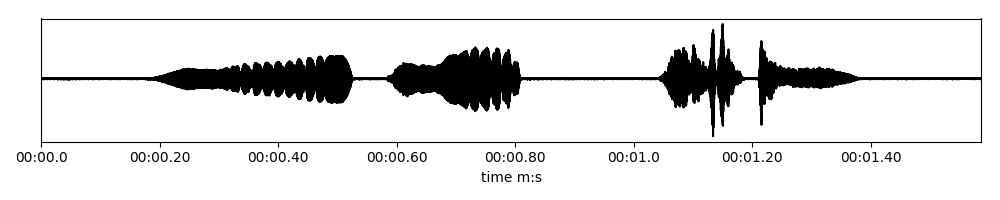
\includegraphics[width=1.0\textwidth]{pcm}
    \caption{}
  \end{subfigure}
  \begin{subfigure}[b]{1.0\textwidth}
    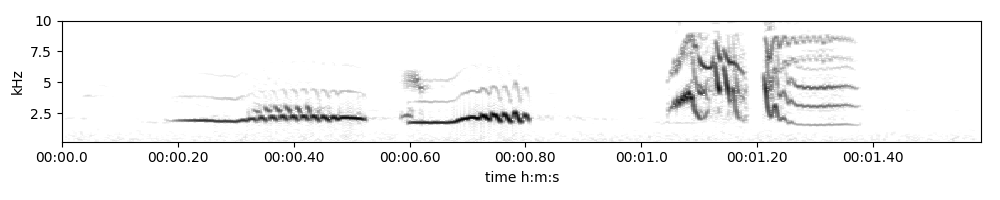
\includegraphics[width=1.0\textwidth]{sgram}
    \caption{}
  \end{subfigure}
  \caption{Waveform (a) and corresponding spectrogram (b) of a bird 1 recording}
  \label{fig:sgram_pcm}
\end{figure}

Our image recognition approach makes use of this spectrographic representation.

Spectrogram construction is performed for all recordings.
This is performed sequentially and immediately stored on disk.
The audio is first loaded as raw pulse-code modulation (PCM).
The windowed fast fourier transform (FFT) method is then used to generate a
spectrogram from the PCM.

Modern hardware handles FFT computations very well, making this stage very quick.
The Matplotlib \parencite{Hunter:2007} |specgram| function is used to generate
spectrograms.

The following parameters are used during spectrogram construction:
\begin{itemize}
  \item \textbf{NFFT}: 512.\\
   Defines the number of PCM data points used in each chunk.
  \item \textbf{Window}: Hann window of 512 points.\\
    Windowing is used to merge overlapping chunks.
  \item \textbf{Overlap}: 75\%.\\
    Overlap defines the number of points overlapping between chunks.
\end{itemize}

Spectrograms are converted to monochrome to simplify operations in the stages
that follow.
This does not reduce the information present in the spectrogram.

Frequencies above 10000Hz and below 100Hz are removed from the spectrograms as
these are less likely to contain relevant vocalisations \parencite{aab}.
These cuts will result in a reduction of baseline noise, as a lot of this falls
under 100 Hz.

\section{Sample Selection}\label{sec:sample_select}
A local database of birdsong samples has been created, using collections
extracted from Xeno-Canto through the described automatic procedure.
Over the course of several days, 2211 total distinct samples have been downloaded
and processed.
189 individual species have been catalogued, with approximately half of these
including more than 10 individual samples.
The top 10 species, and their sample counts are shown in Table~\ref{tab:top10}.
See Appendix~\ref{app:samples} for a full list.
The average length of each recording is approximately 1 minute.

Due to resource limitations imposed by template matching, not all samples
are used in the final evaluation of the algorithm.
Although all samples are processed as described in Section~\ref{sec:prep} and
\ref{sec:preproc}, only a selection is passed through feature extraction and
classification stages.

The following criteria has been found to result in a good balance between
data volume and time cost:
\begin{itemize}
  \item Reject species with less than 20 samples
  \item Retain first 20 samples of each species
  \item Reject species with less than 2000 templates
  \item Keep first 3000 templates of each species
\end{itemize}

To reduce bias samples and templates may instaed be picked at random, however
we did not have time to implement a method for tracking the random sampling.

\begin{table}[!htb]
  \caption{Top 10 species by sample count}\label{tab:top10}
  \centering
    \begin{tabular}{r l}
      Samples & Species Label \\ \hline
      102 & Eurasian Blackcap\\
      101 & Common Blackbird\\
      98  & Eurasian Wren\\
      69  & Common Chiffchaff\\
      66  & Grey-breasted Wood Wren\\
      55  & Spotted Towhee\\
      49  & Garden Warbler\\
      46  & Common Whitethroat\\
      45  & Eurasian Blue Tit\\
      41  & River Warbler\\
    \end{tabular}
\end{table}

The |repository| class facilitates sample rejection and selection based on
several criteria, including class and template counts.

% audio samples (wav): 2211
%  102  Eurasian Blackcap       
%  101  Common Blackbird        
%   98  Eurasian Wren           
%   69  Common Chiffchaff       
%   66  Grey-breasted Wood Wren 
%   55  Spotted Towhee          
%   49  Garden Warbler          
%   46  Common Whitethroat      
%   45  Eurasian Blue Tit       
%   41  River Warbler           
%   40  Great Reed Warbler      
%   39  Rufous-browed Peppershri
%   38  Eurasian Reed Warbler   
%   38  White-breasted Wood Wren
%   38  Yellowhammer            
%   36  Common Grasshopper Warbl
%   35  Northern Mockingbird    
%   32  Common Reed Bunting     
%   32  Corn Bunting            
%   29  Common Cuckoo           
%   28  Common Redstart         
%   27  Common Rosefinch        
%   24  Chestnut-breasted Wren  
%   24  Ortolan Bunting         
%   23  Western Meadowlark      
%   23  Pale-breasted Spinetail 
%   21  European Greenfinch     
%   21  White-throated Toucan   
%   20  Pin-striped Tit-Babbler 
%   19  American Robin          
%   18  Ferruginous Pygmy Owl   
%   16  Barred Antshrike        
%   16  Green-winged Saltator   
%   15  Black-faced Antbird     
%   15  Black-striped Sparrow   
%   15  Lesser Shortwing        
%   14  Plumbeous Vireo         
%   14  Pale-breasted Thrush    
%   14  Plain-tailed Wren       
%   14  Rufous-capped Warbler   
%   14  Swainson's Thrush       
%   14  Channel-billed Toucan   
%   13  White-breasted Tapaculo 
%   13  Common Potoo            
%   13  Tawny Owl               
%   13  Grace's Warbler         
%   13  Greenish Warbler        
%   12  Loggerhead Shrike       
%   11  Great-tailed Grackle    
%   11  Japanese Bush Warbler   
%   11  White-throated Sparrow  
%   11  Collared Owlet          
%   11  Giant Antshrike         
%   11  Undulated Tinamou       
%   10  Rattling Cisticola      
%   10  Painted Bunting         
%   10  Eastern Meadowlark      
%   10  Bell's Vireo            
%   10  Scrub Greenlet          
%   10  Olive Warbler           
%   10  Laughing Falcon         
%    9  Red-winged Blackbird    
%    9  Common Hawk-Cuckoo      
%    9  Yellow-browed Sparrow   
%    9  Slaty-breasted Wood Rail
%    9  Sumichrast's Wren       
%    9  Plain-crowned Spinetail 
%    9  Yellow-eyed Junco       
%    9  Spotted Nightingale-Thru
%    9  Japanese White-eye      
%    8  Southern Yellowthroat   
%    8  Great Tinamou           
%    8  Sooty Antbird           
%    8  Styan's Grasshopper Warb
%    7  Yellow-throated Vireo   
%    7  Connecticut Warbler     
%    7  Hooded Siskin           
%    7  Fire-tufted Barbet      
%    7  Duida Woodcreeper       
%    7  Gartered Trogon         
%    7  Eurasian Treecreeper    
%    7  Buff-browed Foliage-glea
%    7  Eurasian Golden Oriole  
%    7  White-bellied Antpitta  
%    7  Grey Antwren            
%    7  Southern Boubou         
%    6  Recurve-billed Bushbird 
%    6  Golden-crowned Sparrow  
%    6  Splendid Sunbird        
%    6  Moustached Wren         
%    6  Collared Antshrike      
%    6  Violaceous Euphonia     
%    6  Bay Wren                
%    6  Siberian Blue Robin     
%    6  Zigzag Heron            
%    6  Henna-hooded Foliage-gle
%    6  Baillon's Crake         
%    6  Paradise Jacamar        
%    6  Rufous-vented Tapaculo  
%    6  Ashy-headed Greenlet    
%    6  Western Orphean Warbler 
%    6  Spotless Starling       
%    6  Eastern Woodhaunter     
%    6  White-throated Screech O
%    6  Lineated Foliage-gleaner
%    5  Yellow Grosbeak         
%    5  Tanager Finch           
%    5  Foothill Schiffornis    
%    5  Singing Quail           
%    5  Orange-breasted Bushshri
%    5  Esmeraldas Antbird      
%    5  Spectacled Owl          
%    5  Fan-tailed Cuckoo       
%    5  Dark-capped Bulbul      
%    5  Marico Sunbird          
%    5  Yellow-bellied Elaenia  
%    5  Buff-cheeked Greenlet   
%    5  Audubon's Oriole        
%    5  Curve-billed Scythebill 
%    4  White-throated Toucanet 
%    4  Red-fan Parrot          
%    4  California Quail        
%    4  Rufous-tailed Hummingbir
%    4  Black-cowled Saltator   
%    4  Western Wood Pewee      
%    4  Variegated Antpitta     
%    4  Wedge-billed Woodcreeper
%    4  Greater Thornbird       
%    4  Blue-chested Hummingbird
%    4  Green-backed Sparrow    
%    4  Varied Bunting          
%    4  Long-billed Pipit       
%    4  Ferruginous Partridge   
%    4  White-vented Violetear  
%    4  Wedge-tailed Grass Finch
%    3  White-shouldered Antbird
%    3  Blue-winged Pitta       
%    3  White-spectacled Warbler
%    3  Jerdon's Leafbird       
%    3  Olive Thrush            
%    3  Azure Jay               
%    3  Johannes's Tody-Tyrant  
%    3  Short-billed Leaftosser 
%    3  Japanese Quail          
%    3  Chestnut-bellied Thrush 
%    3  Crested Lark            
%    3  Emerald Toucanet        
%    3  Greater Hoopoe-Lark     
%    3  Golden-rumped Euphonia  
%    3  Chestnut-bellied Nuthatc
%    3  Forest Elaenia          
%    3  Moustached Puffbird     
%    3  Choco Tapaculo          
%    3  White-fronted Honeyeater
%    3  White-necked Puffbird   
%    2  Bahama Oriole           
%    2  Arafura Fantail         
%    2  Yellow-crowned Elaenia  
%    2  Plush-crested Jay       
%    2  Scarlet-rumped Trogon   
%    2  Bronzy Jacamar          
%    2  Grey-throated Warbler   
%    2  Pearly Antshrike        
%    2  White-eared Brown Dove  
%    2  Philippine Coucal       
%    2  Flammulated Bamboo Tyran
%    2  Russet Nightingale-Thrus
%    2  Little Cuckoo-Dove      
%    2  White-naped Jay         
%    2  Hepatic Tanager         
%    2  Pririt Batis            
%    2  Solitary Tinamou        
%    2  Black-goggled Tanager   
%    2  Jerdon's Nightjar       
%    2  Cuban Vireo             
%    1  Yellow-breasted Boatbill
%    1  Cherrie's Antwren       
%    1  Sand Martin             
%    1  Negros Scops Owl        
%    1  Yellow-breasted Pipit   
%    1  Curve-winged Sabrewing  
%    1  Streak-breasted Treehunt
%    1  Sombre Rock Chat        
%    1  Mountain Wren-Babbler   
%    1  Eastern Nicator         
%    1  Emei Shan Liocichla     
%    1  Tiny Tyrant-Manakin     
%    1  Crimson-backed Tanager  
%    1  Green-chinned Euphonia  
%    1  Winifred's Warbler      


\chapter{FEATURE SELECTION AND ENGINEERING}

%This section explores possible features in birdsong spectrograms which
%may be used to help identify species.

\section{Useful Feature Identification}
This section explores the information given by the spectrogram image
representation of an audio file, and what features may be extracted to
characterise and identify bird species.

\subsection{Song Segment Formalisms}
Bird song structure is well defined in terms of segmentation \parencite{Catch1997}.
Segment labelling is defined in a naturally descending order of granularity, from
large sequences to basic singular elements, and are identified by their length
and duration of silence between sounds:
\begin{itemize}
  \item \textbf{song sequence:}
    An entire song is a conplete end-to-end sequence of multiple or a single
    phrase.
    The same phrase is may be repeated exactly or with variation within a
    song.
  \item \textbf{phrase:}
    A phrase consists of a series of usually equal syllables.
    Phrases at the end of a song are often not composed of equal syllables.
  \item \textbf{syllable:}
    Syllables may be simple or complex vocalisations.
    Complex syllables can be further partitioned into individual elements.
  \item \textbf{element:}
    Elements form the most basic of vocalisations, for instance, sweeps or tones.
\end{itemize}

\begin{figure}[!htb]
  \centering
  \begin{subfigure}[t]{0.5\textwidth}
    \centering
    \caption{}
  \end{subfigure}
  \begin{subfigure}[t]{0.5\textwidth}
    \centering
    \caption{}
  \end{subfigure}
  \caption{Spectrograms visualising formalised song segments}
\end{figure}

\subsection{Distinctive Features in Spectrograms}
It is common knowledge that bird song is genereally consistent amongst species,
and differ from species to species.
However, there exist some inconsistencies which may become problematic if our
system does not have enough samples to account for the variance.
Specifically, variations exist within a species songs between individuals.

One instance of such variation is regional, where the geographical
location of birds has been found to correlate with nuanced differences in detail.
Local isolation of populations also plays a part in minute variations of song,
referred to as dialects \parencite{podos2007}.

It has also been observed that birds learn aspects of their song, which affects
the exactness of the reproduction \parencite{Krood1983}.
Recordings of younger birds is therefore expected to differ, possibly to a
significant extent.
This is an interesting subject in itself: it is plausable that an automatic
system may be constructed which identifies not only the species of bird but also
an estimate of its age by similar cross-correlation methods.

Birds are able to produce a large varienty of sounds.
These vary from simple pure tones to complex harmonics with amplitude and
frequency modulations \parencite{fager2004}.

Our image recognition approach makes direct use of the structures present
in bird songs.
The intuition is that spectrograms contain all the information necessary to
distinguish a bird song from another, and that these may be segmented and
catalogued such that they form the basis of truth for a statistical
classification system.
Such a system is essentially the automatic equivalent of manual spectrogram 
analysis performed by skilled ornithologists, and somewhat an analogue of natural
pattern recognition done when observing sounds in the field.

Section~\ref{sec:granularity} discusses the issue of selecting an appropriate
granularity for use in cross-correlation.

\subsection{Potential Alternative and Additional Features}
There are a number of potentially useful features which have not been tested or
measured directly in this project.
These are not limited to image recognition approaches, however some are
implicitly included in our approach.

\subsubsection{Variations in amplitude}
Amplitude variations are present in many bird vocalisations.
These have been seen to be dynamic and dependant on the environment and social
context \parencite{brumm2004}
It is therefore likely that this feature is not significantly important for
species recognition.

This feature is however included in the cross-correlation approach since
amplitude is represented in spectrograms, although bearinbg inconsistencies due to
both the dynamic nature of the amplitude variations, and the granularity of the
extracted segments.

\subsubsection{Statistical analysis}
It is possible to extract information regarding the energy distribution in the
spectrogram directly.
Such information may be useful as the difference in song results in observable
differences in fundamental frequencies and bandwidth.
Additionally, it is possible that certain harmonics are characteristic to a
limited number of unique species.

Although not likely to be useful for direct classification of species due to the
existence of similarities between some species, these features may be helpful in
narrowing down the set of possible species, which would save significant time by
reducing the number of cross-correlations needed to exhaustively search for
matching species.

\subsubsection{Segment lengths and repetition frequencies}
Segment statistics such as minimum, maximum and mean duration may be useful to
help identify bird species.
The silence between segments, as well as the repetition rate may also be a
unique or indicative characteristic.

These features are implicitly included through image recognition, but only at
the level of granularity afforded by the template extraction mechanism.
The direct inclusion of extensive segment statistics has been shown to boost
the classification accuracy to some significance \parencite{lasseck2013}.

%\section{Spectrogram Preprocessing}\label{sec:preproc}

Before any features may be extracted, their boundaries must be found.
This is a non-trivial problem due to undesireable noise and recording artefacts
present in each spectrogram.
The problem is considerably worsened by the inconsistency of these from sample
to sample.

The figure below shows an example of a noisy spectrogram.
Notice how the background noise makes it difficult to find the exact boundary of
some of the vocalisations.

show sgram with noise

Even with the quality prefiltering done when downloading recordings from
Xeno-canto, such noise levels remain common.

Because a high number of samples is required for our approach, we developed an
automatic noise reduction stage.
Standard computer vision techinques for noise reduction were used, as well as
techniques for discrete object identification.
A filter is first applied to the spectrogram, which reduces the noise in the
image by smoothing just enough until granular noise is reduced sufficiently (figure x).
The image is then thresholded using an adaptive thresholding algorithm (figure x).
We used adaptive thresholding due to the pixel intensity inconsistencies
throughout some of the spectrogram images.
Further noise reduction is then performed using erosion and dilation which
removes small segments and joins pixel groups which are in close proximity to
each other (figure x).

--\\

global parameters for sweeping noise reductions are suboptimal, what may work
for one recording might not work for another.

yet this is what we do, works ok, specific values were found through trial and
error.

objective is to process spectrograms to find contiguous blobs with similar
scope, that is, either phrases or individual vocalizations.

Some noise reduction steps are semi-automatic, such as adaptive thresholding.

a better approach would be to operate on a per-spectrogram basis, to find the
optimal parameters for each.

This is a non trivial problem.

conceptually the noise reduction algorithm would perform some parameter search
with a heuristic based on the dimensions and quantity of contiguous blobs, with
the aim of reducing the number of small blobs which may resemble noise or disjoint
parts of a single vocalization or segment.

The target scope should be specifiable, so that either individual vocalizations
or complete segments or songs could be extracted.

In some cases it might not be possible to achieve total correct segmentation.

Since different birds have different lengths for specific sounds or parts of song,
the spectral dimensions can not be generalized.
This means that each species will have different aims for quantity and dimensionality,
which must be constructed either by manual input or some feedback mechanism.

a feedback system can then be used to determine which type of segmentation works
best by filtering to various sizes and measuring the accuracy obtained after
classification.

\section{Template Extraction}
Before template images can be extracted for cross-correlation, they must first be
identified in the source spectrograms.
If matching results are to be consistent, spectrograms must undergo
noise reduction and segmentation.
This section details the mechanisms developed for preprocessing spectrogram
images and filtering segments so that only the relevant templates are included for
extraction.

Each spectrogram is processed in sequence using functionality provided by the
OpenCV \parencite{opencv_library} library, and immediately stored on disk.
Parallelisation is possible here, but the computational cost of this stage is
not large enough to have justified sparing development time on this aspect.

\section{Spectrogram Preprocessing}\label{sec:preproc}

Before any features may be extracted, their boundaries must be found.
This is a non-trivial problem due to undesireable noise and recording artefacts
present in each spectrogram.
The problem is considerably worsened by the inconsistency of these from sample
to sample.

The figure below shows an example of a noisy spectrogram.
Notice how the background noise makes it difficult to find the exact boundary of
some of the vocalisations.

show sgram with noise

Even with the quality prefiltering done when downloading recordings from
Xeno-canto, such noise levels remain common.

Because a high number of samples is required for our approach, we developed an
automatic noise reduction stage.
Standard computer vision techinques for noise reduction were used, as well as
techniques for discrete object identification.
A filter is first applied to the spectrogram, which reduces the noise in the
image by smoothing just enough until granular noise is reduced sufficiently (figure x).
The image is then thresholded using an adaptive thresholding algorithm (figure x).
We used adaptive thresholding due to the pixel intensity inconsistencies
throughout some of the spectrogram images.
Further noise reduction is then performed using erosion and dilation which
removes small segments and joins pixel groups which are in close proximity to
each other (figure x).

--\\

global parameters for sweeping noise reductions are suboptimal, what may work
for one recording might not work for another.

yet this is what we do, works ok, specific values were found through trial and
error.

objective is to process spectrograms to find contiguous blobs with similar
scope, that is, either phrases or individual vocalizations.

Some noise reduction steps are semi-automatic, such as adaptive thresholding.

a better approach would be to operate on a per-spectrogram basis, to find the
optimal parameters for each.

This is a non trivial problem.

conceptually the noise reduction algorithm would perform some parameter search
with a heuristic based on the dimensions and quantity of contiguous blobs, with
the aim of reducing the number of small blobs which may resemble noise or disjoint
parts of a single vocalization or segment.

The target scope should be specifiable, so that either individual vocalizations
or complete segments or songs could be extracted.

In some cases it might not be possible to achieve total correct segmentation.

Since different birds have different lengths for specific sounds or parts of song,
the spectral dimensions can not be generalized.
This means that each species will have different aims for quantity and dimensionality,
which must be constructed either by manual input or some feedback mechanism.

a feedback system can then be used to determine which type of segmentation works
best by filtering to various sizes and measuring the accuracy obtained after
classification.


\subsection{Basic Selection and Extraction}\label{sec:template_select}
Given optimal results the segments represent parts of song at the desired
granularity.
This is often not the case however.
Noise may persist after preprocessing, and new deformations may appear, such as
incorrectly joined or incomplete segments.

Some effort is taken to reduce the number of undesireable templates after
preprocessing.
In addition to noise, undesireable templates include extremely specific or
extremely generalised templates.

For example, if a sound is featured in a single instance of bird song, but not
in any other recording of songs of that species, then it is an extreme outlier,
which may occur due to a bird's individual expression or originate from external
sources.
It is non trivial to detect outliers during feature extraction, but because
random forests are generally insensitive to this type of error, we do not
account for these at this stage.

Generalised, or weak templates are easier to detect.
Such templates will have a very faint structure (low contrast), or a complete
lack of structure.
These may be analysed directly and ignored, as they are likely to correlate,
although very weakly, to the majority of spectrograms irrespective of the
species.

Although these rejections bring a theoretical boost to classifier accuracy and
performance, they mainly benefit performance by reducing the number of
cross-correlations computed.

\begin{figure}[h]
  \centering
  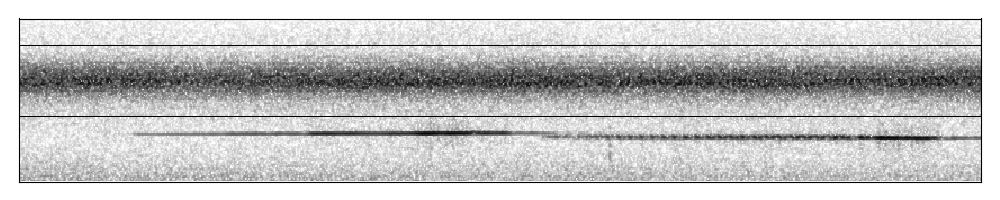
\includegraphics[width=1\textwidth]{large_template}
  \caption{Spectrogram featuring rejected extremely large noise segment}
  \label{fig:bad_select}
\end{figure}

\begin{figure}[h]
  \centering
  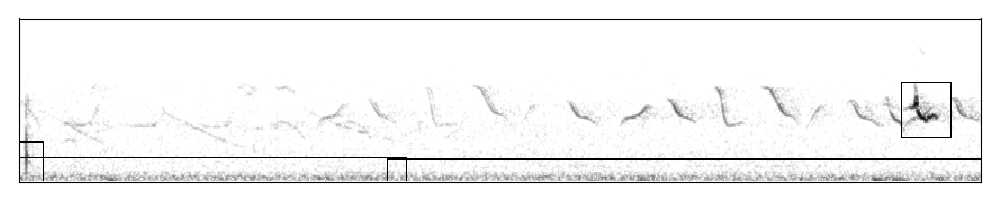
\includegraphics[width=1\textwidth]{bad_select}
  \caption{Spectrogram featuring erronously rejected weak templates}
  \label{fig:bad_select}
  %used XC36327
\end{figure}

\subsubsection{Selection mechanism}
Complete elimination of all undesireable features is impossible without also
removing desireable features.
A balance must therefore be struck, in both preprocessing and selection stages.
Performing selection manually is infeasable given the quantity
of pixel segments.
Selection is therefore done automatically by considering the dimensionality and
pixel values of each template.
Results are shown in Figure~\ref{fig:template_select_effects}\\

Templates with the following properties are automatically rejected:
\begin{itemize}[noitemsep]
  \item \textbf{Area smaller than 50 pixels:} Templates with small dimensions
    are too small to be of any significance and are most likely noise or
    artefacts from preprocessing;

  \item \textbf{Area larger than 10000 pixels:} Templates with extremely large
    dimensions are most likely artefacts from preprocessing, high intensity
    noise or continuous external noises.
    It is possible for sections of song to be merged together into a single
    pixel region due to preprocessing errors.

  \item \textbf{Maximum template intensity lower than average intensity of the
    spectrogram:}
    Low maximum intensity is an indicator background or baseline noise.
    This filter eliminates some of these templates, however not very well.
    Local variance may be a better property to test for, but this has not been
    explored.
\end{itemize}

\begin{figure}[!htb]
  \centering
  \begin{subfigure}[b]{1.0\textwidth}
    \centering
    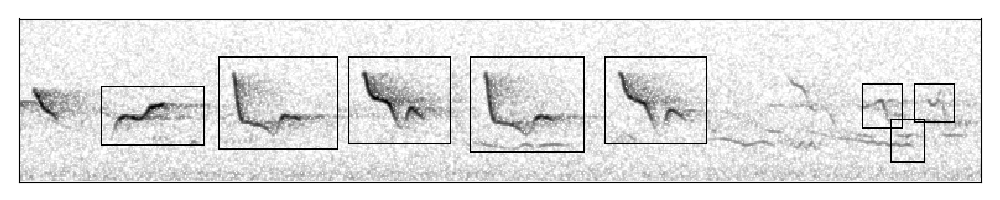
\includegraphics[width=1\textwidth]{accept}
    \caption{}
  \end{subfigure}
  \begin{subfigure}[b]{1.0\textwidth}
    \centering
    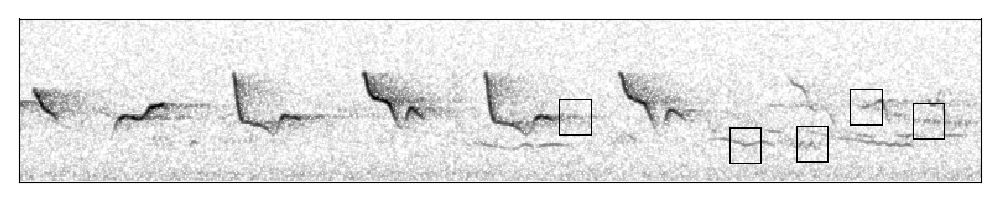
\includegraphics[width=1\textwidth]{reject}
    \caption{}
  \end{subfigure}
  \caption{A noisy spectrgoram showing accepted (a) and rejected (b) templates}
  \label{fig:template_select_effects}
\end{figure}

\subsubsection{Extraction mechanism}\label{sec:extract}

A bounding box is computed for the contours of each segment, which is then used
to extract a template from the original spectrogram image.
Once selection is performed for a particular pixel region, it's bounding box is
expanded by 10 pixels in each direction, and that region is extracted from the
original, unprocessed spectrogram.
This forms a single template.
The template is then blurred using a Gaussian filter with a sigma of 1.5.

Blurring the template allows us to reduce its size, which brings performance
boosts to template matching.
Blurring the template also improves it's generality, which makes matches more
likely.
Care is taken to ensure that templates do not become overly generic, resulting
in ambiguity.
The same operation is made to the spectrograms subject to cross-correlation
mapping for consistency.

\subsection{Advanced Template Elimination}\label{sec:advrem}
It is desireable to reduce the template count further.
This can be made possible by recognizing correlations between candidate templates.
This subsection outlines some speculative methods for
selecting better templates.

\subsubsection{Spatial inclusion}
Imperfections in the preprocessing mechanism leads to errorneous pixel segments.
Incorrect gaps, joins and other inconsistencies in structure persist or
materialise.
If ignored, these are extracted along with valid templates.
If infrequent, the additional templates will factor less as an accuracy penalty,
and more as a performance issue.

In many of these cases, one template's bounding box intersects or is contained
entirely within another template's bounding box as shown in
Figure~\ref{fig:segment_intersect_a}.
These errors can be corrected by taking the bounding box of their unions.
In contrast, Figure~\ref{fig:segment_intersect_b} shows that this does not always
work, and result in large, incorrect groupings.

\begin{figure}[!htb]
  \centering
  \begin{subfigure}[h]{0.5\textwidth}
    \centering
    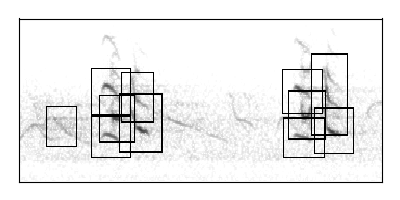
\includegraphics[width=1.0\textwidth]{spatial_fix}
    \caption{}\label{fig:segment_intersect_a}
  \end{subfigure}%
  \begin{subfigure}[h]{0.5\textwidth}
    \centering
    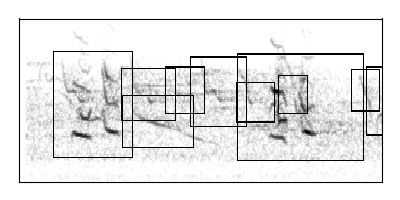
\includegraphics[width=1.0\textwidth]{spatial_unfix}
    \caption{}\label{fig:segment_intersect_b}
  \end{subfigure}
  \caption{Example of errorneous segmentations correctable (a) and incorrectable (b)
  by merging their bounding boxes}
  \label{fig:segment_intersect}
\end{figure}

\subsubsection{inter-template correlation}
As expected, templates will have some level of inter-correlation.
This leads to a database of many hundreds or thousands of very similar templates.
Merging these in some form has been considered but not approached.
This would benefit performance dramatically, but it is most likely to cause
a noticeable dip in accuracy.
For this to succeed, the result of the merge must represent all related templates
equally, and it is clear that this would not be as accurate as individual
templates.

It can also be argued that templates with little to know intercorrelation may be
independent anomalies, such as noise or external signals irrelevant to the
subject species.

\subsubsection{Species-specific template statistics}
It may be possible to use information regarding average dimensionality and mean
frequency information to determine the relevance likelyhood of a particular template.
Such metrics require an existing set of validated templates, which may be gathered
by filtering a non discriminated set of templates by their measures importances.

Figure~\ref{fig:bandlimit} shows how the birdx song doesn't use vocalisations
under 123 Hz.

\begin{figure}[!htb]
  \centering
  \caption{Example of a bird song with a principal frequency range}
  \label{fig:bandlimit}
\end{figure}

\section{Feature Engineering}
With the collection of extracted templates from each spectrogram,
a model can now be constructed for a particular sample.
This model is represented as a feature vector consisting of the maxima
of each template cross correlation operation done on the spectrogram.
This vector will then be compared to those of other samples using a
classifier.
This section describes in detail the operation of template matching
to build this feature vector, as well as some notes on the time
required.

\subsection{Cross-correlation Mapping}
Cross-correlation mapping, also referred to as template matching, is
a method for determining the similarity of an image within another,
often larger image.
It is essentially a form of image recognition.
The intuition is that songs from birds of the same species will have
extremely similar spectral shapes.

Cross-correlation mapping works by convolving the template image
over the target image and measuring the pixel similarities.
check this.

The Open-CV library is used to perform template matching.
Open-CV's implementation is highly optimized, and may be computed
using a GPU. For details see appendix.

\subsubsection{Results}
The result of template matching is a cross-correlation mapping of the
template against the target spectrogram.
show an example of a template ccm against a spectrogram.

The data in the mapping can give us a rough estimate of how closely
the template matches.
Given this result, we store the global maxima of the mapping in a
feature vector.

\subsection{Feature Vector Construction}
When classifying a particular sample, the spectrogram is cross-correlated
with each template accumulated so far in the database.
For each cross-correlation, the maxima of the result is taken and stored
at the index in the vector correspoinding to the template that was used.
We then refer to this index later for further analysis.

\subsection{Computational Expense and Optimizations}
Template matching is the most expensive operation in the program.
Although the underlining algorithm is itself well optimized, further
improvements can be made for marginal gains.

\subsubsection{Time anal}
Template matching takes approximately x minutes per template, given
mean dimensions of mxn and ixj for spectrograms and templates respectively.
Considering the quantity of templates stored in the database, the time
required quickly compounds into the order of days.
xx templates against yy spectrograms was measured at x days on a xyz machine.
This stresses the requirement for optimization, which is the topic of
section blah.

\subsubsection{Implemented and proposed optimizations}
Dimensionality reduction:
Correlation area truncation:


\chapter{CLASSIFICATION AND EVALUATION}

\section{Random Forests}

\section{Accuracy Evaluations}

\section{Classification}
With feature vectors constructed, we select a machine learning algorithm to
train and classify birdsong based on our model.
This section details the choice of algorithm, it's variations, performance and
tuning.

\subsection{Approaches to Classification}
obviously a classification task.
We are working with limited sample set, but high number of features.
The data is labelled, so we will select a supervised learning algorithm.
we must select a classifier which performs well with this data.
identifying the best classifier can be best done by cross validating each and
selecting the best performer.
For the purposes of testing our approach, a single algorithm was initially
chosen.

random forest is a good performer and is highly scalable (ref).
We chose this algorithm.

also might look at gradient boosted trees.

number of classifiers can be used
skim through some strengths and weaknesses

\subsection{Random Forest Classifier}
A random forest classifier is an ensamble of trees.
A node of a tree is split on an index of the feature vector.
Each Tree uses a new random sampling of the features.

we pick the random forest.
explain why we use this classifier
explain how it fits with the data we are working with

This is a multi-class classifier, returning the probabilities of each class
corresponding to the data given.
An alternative approach is possible, in which the classification of each species
is split into individual random forests, the final result of which is retrieved
by taking the maximum of all probabilities.
Using multiple binary classifiers allows other accuracy metrics to be used,
facilitating the accuracy evaluation of single species.

\subsubsection{Extremely Randomised Trees}
Extremely Randomised Trees is similar to a traditional Random Forest, however
however splitting is randomised, instead of being computed for optimal
performance.
This has the benefit of being faster, with the drawback of being more sensitive
to noisy features.\\

Using this classifier has seen no major accuracy or performance differences.
why do we use it, no reason??

ert thresholds are random, best one is picked, reduces variance, increases bias

\subsection{Parameter Selection}
show parameters available for RF
show initial parameters chosen and their performance
how did we pick these? (make something up)

Section~\ref{sec:tuning} explores semi-automatic parameter tuning and touches on
the issues of overfitting.

\section{ Evaluation and Validation}\label{sec:acc_eval}
To validate our model, several metrics are taken to measure the performance of
our model.
Although random forests are less likely to overfit, it can still occur, and is
nonetheless important to detect.

Most metrics, natively suited to binary classifiers, are easily adapted for use
in multi-class tasks.
It is equally important to correctly sample the data as to avoid bias.
This section discusses first the framework around which the performance of our
model is measured, the metrics used, and finally an analysis of the results.

Section~\ref{sec:tuning} analyses the performance of the classifier with varying
parameters, in order to find their optimal values.

\subsection{Validation Strategy and Sample Space}
In effort to reduce sensitivity to chance selection of random samples, all
measurements are performed using a multi-run stratified 10-fold cross validation.
This gives us a 90/10 train/test data split, and is repeated with a new random
sample shuffling 10 times.
Stratification ensures that there exists an equal class balance in the testing
and training splits, so that all classes are represented equally.

This is especially important given the small number of representative samples
for each class.
Advanced methods exist in order to futher improve our results, such as
bootstrapping, but this has not been pursued.
Note that random forests use bootstrap sampling, where a portion of the data is
not used for training.
This does produce a measurable result similar in effect to cross-validation,
called the OOB error, discussed in Section~\ref{sec:metrics}.

For each fold, only features from the selected training samples are
used for training and validation.

A total of 3 batches have been computed and merged, giving 12 species in total.
Selection was performed using the mechanisms outlined in
Section~\ref{sec:sample_select}.
Table~\ref{tbl:used_data} shows the selection of species including spectrogram
and template counts per species.

\begin{table}[!htb]
  \caption{Selected species with spectrogram and template counts}
  \label{tbl:used_data}
  \centering
  \begin{tabular}{l r r}
    Species Label & Spectrograms & Templates \\ \hline
    Common Blackbird           & 20 & 6132\\
    Great Reed Warbler         & 20 & 5111\\
    Common Rosefinch           & 20 & 3191\\
    Common Cuckoo              & 20 & 2909\\
    Common Chiffchaff          & 20 & 2886\\
    European Greenfinch        & 20 & 2759\\
    Pale-breasted Spinetail    & 20 & 2501\\
    Ortolan Bunting            & 20 & 2362\\
    Common Reed Bunting        & 20 & 2233\\
    Chestnut-breasted Wren     & 20 & 2203\\
    Corn Bunting               & 20 & 2082\\
    Rufous-browed Peppershrike & 20 & 1404\\ \hline
    \multicolumn{1}{r}{Total} & 240 & 35773
  \end{tabular}
\end{table}

\subsection{Evaluation Metrics}\label{sec:metrics}
Each of the five following evaluation metrics are computed in a fold.
They are then stored and averaged at the end of the cross validation.

\begin{itemize}
  \item \textbf{Accuracy}
    Is the ability of the classifier to correctly label samples.
    \begin{equation}
      \frac{TP+TN}{P+N}
    \end{equation}

  \item \textbf{Precision},
    Sometimes referred to as the positive predictive value, is the ability of the
    classifier to label all predicted values correctly.
    \begin{equation}
      \frac{TP}{TP+FP}
    \end{equation}

  \item \textbf{Recall},
    Sometimes referred to as sensitivity, is the ability of the classifier to
    label all positive samples correctly.
    \begin{equation}
      \frac{TP}{P}
    \end{equation}

  \item \textbf{F-beta score}
    Is the weighted harmonic mean of the precision and recall, where
    higher values indicate better performance.
    This makes it simpler to compare the performance of different parameter sets.
    \begin{equation}
      \frac{(1+\beta^2)TP}{(1+\beta^2)TP+\beta^2FN+FP}
    \end{equation}

    We consider precision and recall as equally important, in which case the
    beta value is set to 1:
    \begin{equation}
      \frac{2TP}{2TP+FN+FP}
    \end{equation}

  \item \textbf{OOB error rate}
    Is the out-of-bag (OOB) samples are those which were not selected during the
    construction of a specific tree.
    Given the most common label from classifying a sample with its respective tree,
    the porportion of incorrect classifications is averaged over all OOB samples
    is taken as the OOB error rate on the training data.

\end{itemize}

The Scikit Learn |precision_recall_fscore_support| function was used to compute
these metrics.

Because this is a multi-class classification task, each metric is computed
on a per-label basis.
The average is then computed using "macro" averaging, in which the mean of each
score is computed with equal weighting for all labels.
This is appropriate considering we use stratified k-fold, and each
species is considered equally important to all the others.

\subsubsection{Results}
Results are promising, good performance has been achieved using the initial
parameters, with observed improvements after tuning as is shown in
Table~\ref{tbl:acc_before_after}.

\textbf{update w/ new defaults}
\textbf{wait for gs results... }
\begin{table}[!htb]
  \centering
  \caption{Comparison of accuracies using default and tuned parameters}
  \label{tbl:acc_before_after}
  \begin{threeparttable}
    \begin{tabular}{l r r}
      & \multicolumn{2}{c}{Metric Scores} \\
      Metric    & Default Params. & Tuned Params. \\ \hline
      Accuracy  & 79.5 (7.3) & 0 \\
      F1 Score  & 77.9 (8.1) & 0 \\
      Recall    & 79.5 (7.4) & 0 \\
      Precision & 82.3 (8.5) & 0 \\
      OOB Error & -- & --
    \end{tabular}
    \begin{tablenotes}
      \footnotesize
      \item[*] Values are shown as percentages.
      \item[*] Standard deviations are shown in parentheses.
    \end{tablenotes}
  \end{threeparttable}
\end{table}

\subsection{Confusion Matrix}
A confusion matrix plots the rate at which each label is predicted as any other
label, where the rows represent the true label, and columns represent the
classifier's predictions.

We construct a confusion matrix to evaluate the performance of the classifier
and the features used to discriminate between species.
In this case the matrix allows us to visualise the performance distribution per
class, and give
some insight into how the classifier is responding to the selected features.

Figure~\ref{fig:cnf12} shows the resulting confusion matrix from classifying the
selected data, averaged over the 10-run 10-fold cross validation.
Row-wise normalisation was performed.

\begin{figure}[!htb]
  \centering
  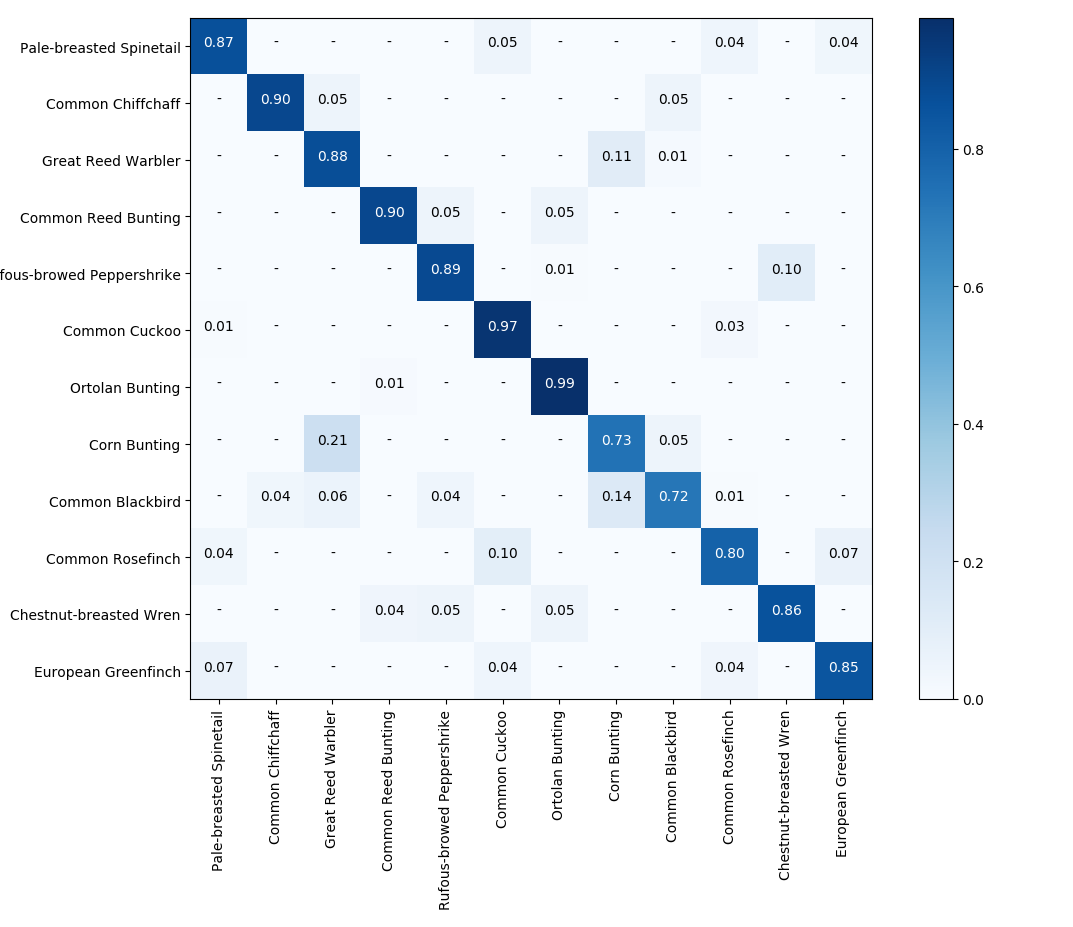
\includegraphics[width=1.0\textwidth]{cnf_matrix_12}
  \caption{Row-Normalized Confusion Matrix}\label{fig:cnf12}
\end{figure}

The confusion matrix shows good classification performance for most species.\\

We can see from the results that the Common Blackbird is the worst performing
classification with a 40\% false negative rate.
It is often mistaken for a Great Reed Warbler, but not the other way around,
which may indicate weakness in the Common Blackbird's templates.

... more speculation

Aside from computing the metrics shown in Section~\ref{sec:metrics}, a confusion
matrix can only offer a speculative insight into template performance.
Nonetheless, it offers a starting point into further template analysis as
discussed in Section~\ref{sec:template_analysis}.

\section{Feature Importance}\label{sec:feature_imp}
Because our feature vector is directly related to the templates of each species,
it is possible to determine their role and effectiveness in classifying a
recording by computing feature importances from our classifier.
This allows us to reduce the number of templates involved in classifying a given
sample, significantly cutting down the cost of template matching per species.
Feature importances also help us analyse the preprocessing performance in detail,
as well as correlate inter-species similarities in cases where there is a high
level of confusion.

\subsection{In Random Forests}

\subsubsection{Mean decrease accuracy}
One method for measuring the impact of each feature is through the mean decrease
in accuracy.
With this method, the impact of removing each feature one-by-one is measured.
This method may be sensitive to the random nature of the classifier, so multiple
runs may be required to eliminate any variance (is this true?).
This can be prohibitively expensive.

\subsubsection{Mean decrease impurity}
Because the nodes of trees in a random forest correlate directly with a specific
feature, it is possible to directly measure or estimate the importance of each
feature by determining the probability of a node in a tree being traversed over 
the number of nodes in the forest.
This is known as the mean decrease impurity, or gini importance, which is what
is used in Sckikit's random forest classifier implementation.

\subsection{Results and Analysis}

Measuring feature importances exposes an average of x out of 3000 samples as
completely irrelevant during training and classification.
Removing these features shows no reduction in accuracy, and a significant speedup
during template matching is gained, reducing total classification time from 10000
hours to 0.5 seconds.

There are 1209301293123 templates distributed across 20 spectrograms for each
of the 50 species selected.
When clsasifying a new sample, it's spectrogram must be cross-correlated with
each of the templates.
This operation is extremely expensive, in the order of 42 hours, or 25 seconds
per template of average dimensions (125x125) with a target sample of average
length (3 minutes). (see apndx 1 for detailed time analysis)

The aim is therefore to reduce the feature count as much as possible while
retaining the highest possible accuracy by determining an appropriate importance
cutoff.
Removing features and reevaluating the classifier takes no significant time in
contrast to template extraction and may therefore be done by iteratively removing
and checking classifier accuracy, adjusting the importance cutoff accordingly.
Measuring feature importance unfortunately requires a complete run which involves
the cross-correlation of all templates, which negates any performance benefits
for recordings which aren't new to the system.
Since we are using cross-validation to evaluate all samples, all templates are
used eventually, even if their importances remain low across all folds.\\

Feature reduction is very helpful during feature extraction, when merging the
results of two batches.
Templates with importance scores equalling or close to zero can be safely removed
from the set before merging, saving a considerable amount of time.
Time saved is estimated to be 232103 minutes on average.

\textbf{unless we can get importances from training only, then when we test
we can use the reduced template set and speed all this up}

\textbf{graph of feature importances}\\


\textbf{paragraph on important and non important feature analysis. lots of 
images, look at templates belonging to confused species, try to determine
which are culprits, probably most of them}

\section{Classifier Tuning}
we havent done this.
section talks about the importance of tuning the classifier for
optimal performance.
touches on issues of overfitting.


\subsection{Gridsearch}
explain gridsearch and how to use it.
explain how we use it if we do.

\subsection{Parameter Analysis}
Analuse the results of parameter optimization
also measure overfitting



\bibliography{refs}
\bibliographystyle{alpha}

\appendix
\include{app_}

\end{document}
